\documentclass[a4paper,11pt,twoside]{article}

%%%%%%%%%%%%%%%%%%%%%%%%%%%%%%%%%%%%%%%%%%%%%%%%%%%%%%%%%
%%
%% Dit is de instructie voor ABI studenten aan de OU.
%%
%% Het huidige bestand is gebaseerd op XeLaTeX en
%% rendert naar een PDF file.
%%
%% De output richt zich op tweezijdig afdrukken. Als gevolg
%% daarvan is de marge van elke pagina gespiegeld.
%%
%% Mocht je 1-zijdig willen afdrukken genereer dan de pdf
%% file zonder de optie ``twoside'' in documentclass.
%%
%%%%%%%%%%%%%%%%%%%%%%%%%%%%%%%%%%%%%%%%%%%%%%%%%%%%%%%%%

%%
%% Uncomment de includeonly en vul de hoofdstukken in die je
%% in PDF wilt zien. Zet er een % voor als je alle hoofdstukken wilt zien.
%% Als je meer onderdelen wilt zien, maak dan een eigen comma separated list.
%%
%\includeonly{ov-abi-instructie-overview}
%\includeonly{ov-abi-instructie-overview, f1-abi-instructie-fase1}

\usepackage{ucs}
%\usepackage[utf8]{inputenc}
\usepackage{subfigure}
\usepackage[dutch,english]{babel}
\usepackage{graphicx}
\usepackage{wrapfig}
\usepackage{hyperref}
%\usepackage{paralist}% for compact lists: compactenum, compactitem
\usepackage{supertabular}
\usepackage{dingbat}% for \leftpointright

\author{Guus Bonnema}
\title{ABI Instructie}
\date{20/09/14}

\begin{document}
\selectlanguage{dutch}

\tableofcontents

%%
%% Dit is een onderdeel van abi-instructie.tex
%%
\section{Projectstappen op hoofdlijnen}

De activiteiten binnen ABI kunnen in een viertal fasen opgedeeld worden.
De eerste twee fasen hebben te maken met de voorbereiding van het voor de
opdrachtgever uit te voeren project. De fase 3 betreft de uitvoering van dit
project en de fase 4 de afronding.

\begin{figure}[!ht]
    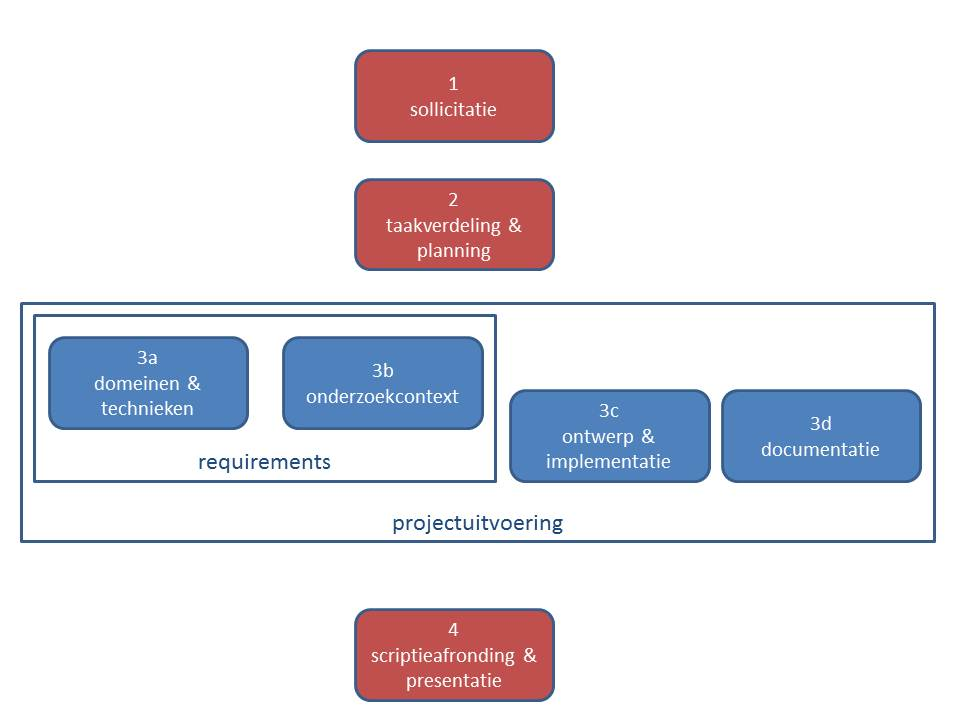
\includegraphics[width=\textwidth]{./overview.jpg}
    \label{fig:overview}
    \caption{De globale planning: overview}
\end{figure}

Voor elk van de fase 2 en 4 en de deelfasen 3a t/m 3d staat een nominale
doorlooptijd. Elk van deze fasen wordt afgesloten met een mijlpaaldocument
dat kwalitatief beoordeeld wordt door de begeleider. Alleen de fase 3a
wordt afgesloten met een individueel mijlpraaldocument,  de overige mijlpaalproducten
zijn groepsproducten.

Het eindcijfer wordt bepaald door de examinator, rekening houdend met de
kwalitatieve beoordelingen van de begeleider.

Gedurende het gehele proces vindt er tenminste een (virtueel) maandelijks
overleg plaats tussen het gehele team en de begeleider. Input voor dit
overleg zijn de individuele maandrapportages en de eventuele mijlpaaldocumenten
die u in de afgelopen maand opgeleverd heeft.

Van elk mijlpaaldocument worden slechts 2 versies door de begeleider
beoordeeld. Op een conceptversie ontvangt u feedback met
verbetervoorstellen en de tweede versie wordt beoordeeld.

\begin{figure}[!ht]
    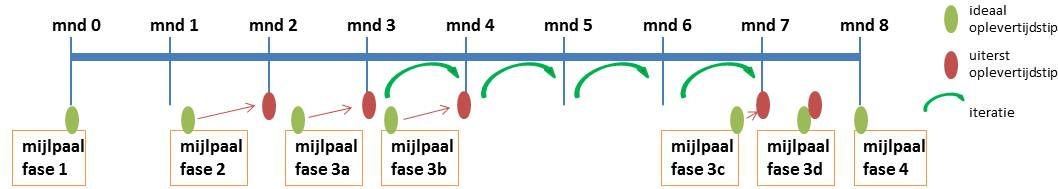
\includegraphics[width=\textwidth]{./globale-tijdsplanning.jpg}
    \label{fig:globale-planning}
    \caption{De globale planning: volgorde van mijlpaalproducten}
\end{figure}

Afbeelding \ref{fig:globale-planning} geeft een indicatie omtrent de
opleveringtijdstippen van de verschillende mijlpaalproducten na de
start van het ABI-project. Groene bolletjes geven de ideale
oplevertijd weer en rode bolletjes de uiterste oplevering
per mijlpaalproduct.

Ook zijn de mogelijke iteraties getoond maar het aantal
iteraties en de duur van een iteratie bepaalt u als team
in overleg met de opdrachtgever.

\subsection{Voorbeeldplanning}
Een ``ideale'' planning bij een start in september dan wel februari
ziet er als volgt uit.

Deze planning geeft een beeld van de verhouding tussen de inspanningen
in de verschillende fasen.Uiteraard maakt u als team in fase 2 een eigen
planning en er kunnen allerlei goede redenen zijn om af te wijken van
de ideale planning. Zeker de activiteit 3c vraagt ook om een nadere
uitsplitsing; bv. in de vorm van sprints van 3-4 weken. Ook is het
raadzaam om in fase 2 al na te denken over een mogelijke einddatum
van het project waar als team naartoe gewerkt wordt zodat de verwachtingen
bij alle betrokkenen helder zijn.
De midterm bijeenkomsten zijn medio november en medio april.

%%
%% De voorbeeld planning runs op het web kloppen niet, zijn inconsistent.
%% Met name de voorbeeld duren en start en eindtijd van de 3b, 3c en 3d
%% subfasen zijn vreemd. De volgorde klopt ook niet. Enigzins aangepast, maar nog niet correct.
%%
%%

\begin{framed}
    \begin{center}
	\begin{tabular}{lllr}
	    \textbf{fase} & \textbf{doorlooptijd} & \textbf{voorbeeld} & \textbf{netto}\\
	    fase 2        & 1.5  & medio sept - eind okt & 20\\
	    fase 3a       & 2    & eind sept - eind nov & 50\\
	    fase 3b       & 2    & eind nov - eind dec & 30\\
	    fase 3c       & 5    & eind nov - eind apr & 230\\
	    fase 3d       & 2    & eind mrt - eind apr & 50\\
	    fase 4        & 1.5  & eind mrt - medio mei & 20\\
	\end{tabular}
    \end{center}
    \captionof{table}{Run vanaf september}
 \label{fig:sept-run}
\end{framed}

\begin{framed}
    \begin{center}
	\begin{tabular}{lllr}
	    \textbf{fase} & \textbf{doorlooptijd} & \textbf{voorbeeld} & \textbf{netto}\\
	    fase 2        & 1.5  & medio febr - eind mrt & 20\\
	    fase 3a       & 2    & eind febr - eind apr & 50\\
	    fase 3b       & 2    & eind mrt - eind mei & 30\\
	    fase 3c       & 5    & eind apr - eind sept & 230\\
	    fase 3d       & 2    & eind mrt - eind sept & 50\\
	    fase 4        & 1.5  & eind sept - medio okt & 20\\
	\end{tabular}
    \end{center}
    \captionof{table}{Run vanaf februari}
 \label{fig:febr-run}
\end{framed}

%%
%% Dit is een onderdeel van abi-instructie.tex
%%
\section{Fase 1 Sollicitatie}
De sollicitatiefase omvat de activiteiten die voorafgaan aan ABI.
Voordat u met ABI kunt beginnen dient u zich in te schrijven maar
u dient zich ook aan te melden bij de examinator. Deze bepaalt op
basis van de informatie die u verstrekt over uw studieresultaten
en uw planning of u toegelaten kunt worden tot een bepaalde run
van ABI.

Hebt u toestemming gekregen van de examinator dan kunt u
deelnemen aan de startbijeenkomst. De startbijeenkomst is virtueel,
via Collaborate (voorheen Elluminate). Deelname aan deze bijeenkomst
is verplicht. Bent u om welke reden dan ook
verhinderd, meldt dit dan ruim vooraf aan de examinator Marko
van Eekelen en de co\"{o}rdinator Frans Mofers.

De datum van de eerstvolgende startbijeenkomst wordt bekendgemaakt
via de mededelingenpagina van de cursus in Studienet . Plaats het
ingevulde voorstelformulier uiterlijk 3 dagen voor de startbijeenkomst
in de discussiegroep. Zorg wel dat u tijdig voor de startbijeenkomst
kunt beschikken over een headset en bij voorkeur ook een webcam.
Informatie over het gebruik van Elluminate treft u aan in de help van Studienet.

Wanneer u geen ervaring met Collaborate heeft, dan kunt u een half uur
voorafgaand aan de startbijeenkomst, het functioneren van apparatuur
en programmatuur testen met ondersteuning. Uit ervaring blijkt dat het
testen van het geluid geen overbodige luxe is wanneer u niet regelmatig
met Skype of andere hulpmiddelen werkt.

Houd ook uw email inbox in de gaten omdat in geval van calamiteiten
daar berichten uitgewisseld zullen worden. Tijdens de startbijeenkomst
krijgt u uitleg over het project, kiest u teamleden om het project samen
mee uit te voeren, en kiest u als team \'e\'en van de beschikbare projecten.

Op Studienet (onder Mededelingen) kunt u kennis nemen van de projecten
waaruit u kunt kiezen voor een bepaalde run. U vult een aantal dagen
voor de startbijeenkomst het voorstelformulier in en plaatst het
ingevulde formulier op het forum bij de cursus op Studienet.
U bestudeert uiteraard de instructie op Studienet en woont de (virtuele)
startbijeenkomst bij. Tijdens de startbijeenkomst vormt u een team.
Elk team kiest een project.

Bij de teamvorming en de keuze van de projecten wordt gelet op de
voorkennis, de individuele voorkeur voor bepaalde projecten en wordt
gekeken naar de beschikbare tijd per week. De teams zullen uit ongeveer
drie teamleden bestaan.

De examinator is de uiteindelijk verantwoordelijke voor de
teamsamenstelling en de projectkeuze. Aan een team wordt een
begeleider gekoppeld met vakinhoudelijke kennis. Vervolgens neemt u
contact op met de opdrachtgever en u stuurt naar uw begeleider
uw voorlopige competentiekeuze.

%%
%% Dit is een onderdeel van abi-instructie.tex
%%
\section{Fase 2 Taakverdeling \& planning}
\subsection{Inleiding}
In deze fase verzamelt u de benodigde informatie en maakt u afspraken
binnen het team als ook met de opdrachtgever. Het doel van de activiteiten
in deze fase  is het samenstellen van een helder mijlpaalproduct waarin u
de kaders en de aanpak vastlegt voor het uit te voeren project.

U gaat na waar precies de problemen zitten bij de opdracht, legt op
hoofdniveau de requirements vast, maakt een globale architectuurkeuze
en gaat na welke toolalternatieven er zijn, welke toolkeuze u al kunt
maken en welke nog niet in deze fase maar in het vervolg van het project
gemaakt zullen moeten worden (bv. via de domeinanalyse in fase 3a).

Over het algemeen zult u iteratief te werk gaan, en de requirements
gedurende het project verfijnen en aanvullen, maar in deze deelfase
beschrijft u de requirements op hoofdlijnen.

De eerste iteratie beschrijft u bij voorbaat al in detail in het
plan van aanpak en de andere beschrijft u globaal. Ook
geeft u aan hoe u de fasen 3a en 3b denkt aan te pakken.

Voor uw projectplan is van belang dat u verschil maakt tussen de
ontwikkelmethode die u gaat hanteren en de planning van het project
die u uit gaat voeren. De ontwikkelmethode beschrijft de principi\"ele
aanpak en in de projectaanpak legt u vast op welke manier u in uw
project met de ontwikkelmethode om  zult gaan. Voor wat betreft
de ontwikkelmethode wordt een iteratieve methode aanbevolen gezien
het innovatieve karakter van de meeste projecten.

Om binnen het team goed afspraken te kunnen maken over de rollen
in het project, communiceert u met elkaar de competenties die u
wilt uitoefenen in het project.

\subsection{Doelstelling}
    In deze fase voert u overleg met uw teamleden, de opdrachtgever en de
begeleider over de manier waarop u het project gaat aanpakken. U wordt het eens
over de taakverdeling, eventuele onduidelijkheden in de opdracht zijn weggenomen
en u legt vast hoe u de uitvoering aan gaat pakken. Dit legt zowel de keuzen
die u in dit stadium kunt maken vast als dat het expliciet maakt voor welke
aspecten u in de vervolgfasen nog keuzen zult moeten maken.
    U gaat na waar precies de problemen zitten, legt op hoofdniveau de
requirements vast en de aanpak die u zult doorlopen. U denkt het project
procedureel door maar vooral ook inhoudelijk en gaat na waar u de grootste
uitdagingen verwacht aan te treffen. U beschrijft de globale architectuur en de
toolalternatieven.

\subsection{Stappen}

\paragraph{Team overleg}
U spreekt af met uw teamleden hoe vaak, en op welke manier, u met elkaar
overlegt. Het is uiteraard aan te bevelen daar een vaste afspraak
voor te maken.
\paragraph{Begeleider overleg}
U spreekt af met uw begeleider hoe vaak u hem of haar voor de
bijeenkomsten uitnodigt. Een handige manier is om bijvoorbeeld
wekelijks
teamoverleg te hebben, en daarbij maandelijks te begeleider uit te
nodigen.
\paragraph{Taakverdeling}
U stelt een onderlinge taakverdeling op. Daarbij is het van belang dat u
niet uitsluitend werkzaamheden kiest waarmee al ruim ervaring
opgedaan heeft, maar juist ook taken kiest waarbinnen u één of
twee competenties kunt ontwikkelen. U legt de definitieve competentiekeuze
vast en relateert deze aan uw taken in het project.
\paragraph{opdrachtformulering onderling}
U bespreekt onderling of er onduidelijkheden in de opdracht zijn. Op dit
moment kunt u nog niet de requirements in detail vast gaan leggen:
dat gebeurt
in fase 3. Wel kunt u op dit moment bekijken of u voldoende
informatie heeft om in fase 3 aan de slag te gaan met domeinanalyse,
bestuderen van relevante tools en technieken, en het helder krijgen
van requirements.
\paragraph{Aanpak}
U bespreekt onderling hoe u te werk zult gaan. Daarbij is van belang
welke ontwikkelmethode u zult gaan gebruiken. Voor een klein team
met een opdracht met veel onbekenden ligt een agile/iterative aanpak
voor de hand, maar daarvoor is instemming van de opdrachtgever nodig.
\paragraph{Opdrachtformulering}
U bespreekt met de opdrachtgever (meestal per e-mail) de
onduidelijkheden in de opdracht, en de rol die de opdrachtgever
tijdens het project zal spelen.
U gaat met de opdrachtgever na of deze een prototype wil of een
(volledig) operationeel systeem dat door eindgebruikers gebruikt kan
worden.
\paragraph{Projectplan}
U legt alle genomen beslissingen vast in een projectplan (u kunt daarbij
gebruikmaken van het boek Praktisch Projectmanagement 1 dat u bij
inschrijving heeft ontvangen) en in een overeenkomst met de opdrachtgever. In het
projectplan legt u de context van het project vast, het probleem dat u gaat
oplossen of een kans die u gaat creëren middels dit project alsmede de doelstelling
van het project. Ook legt u de uitgangspunten en randvoorwaarden vast.
In het projectplan kunt u op dit moment nog niet exact vaststellen wat u
gaat opleveren, omdat u pas in de volgende fase de requirements
helder kunt krijgen. U zult ook de tijdsplanning en de ontwikkelaanpak
slechts globaal kunnen beschrijven.
\paragraph{Architectuur}
U legt in een algemeen architectuurplaatje de context van het beoogd
informatiesysteem vast.
\paragraph{Aanbevolen}
Teneinde het ABI project planmatig en tijdig af te kunnen ronden bevelen wij
u sterk aan de ontwikkelmethode te kiezen die beschreven staat onder het kopje
Ontwikkelmethode.

\subsection{Onderdelen mijlpaalproduct}
    Het mijlpaalproduct voor fase 2 omvat de volgende onderdelen:
\begin{itemize}
    \item de achtergronden van het project, de opdracht en het beoogde resultaat
(het ambitieniveau)
    \item de planning van de activiteiten (de opdeling in fasen) met hun mijlpalen
    \item de inzet van de teamleden en hun rollen en de te gebruiken hulpmiddelen
    \item het test- en documentatieplan
    \item de benodigde hulpmiddelen
    \item de projectrisico’s en mogelijke maatregelen voor risicoreductie
    \item de maatregelen voor kwaliteitsbewaking (op product en proces!)
    \item de voorlopige keuze van het onderwerp dat elk teamlid specifiek zal
	    onderzoeken in de fase 3a: domein \& technieken
    \item een korte afbakening van het probleem
    \item de specifieke onderzoeksvraag die via het domeinonderzoek beantwoord
	    dient te worden
    \item de manier waarop u kennis wilt vergaren over de onderzoekcontext en hoe
	    u deze kennis zult documenteren
    \item de manier van communiceren (binnen het project en met de opdrachtgever)
    \item een globale architectuurschets van de belangrijkste componenten van het
	    te ontwikkelen systeem in zijn omgeving
    \item een lijst met relevante begrippen
    \item de overeenkomst met de opdrachtgever.
\end{itemize}

\subsection{Rol begeleider}
    De begeleider zal feedback geven op de aanpak die u voorstelt voor het
project.
    Indien daar aanleiding toe is zal de begeleider ook aangeven dat u nog
stukken theorie dient te bestuderen rond competenties die mogelijk nog
onvoldoende ontwikkeld zijn. Voorbeelden van competenties waaraan in ABI op
basis van een individuele beoordeling extra aandacht besteed kan worden zijn:
plan opstellen, presenteren, samenwerken, schrijven of literatuur zoeken.
    U stuurt maandelijks een kort overzicht op van de voortgang. Het is aan te
bevelen om maandelijks overleg met de begeleider te plannen, en het
voortgangsoverzicht kort daarvoor op te sturen.
    U stuurt een conceptversie van het mijlpaalproduct op naar uw begeleider. De
begeleider geeft commentaar, en u kunt eventueel aan de hand daarvan wijzigingen
aanbrengen en stuurt de definitieve versie voor beoordeling naar de begeleider.

\subsection{Ontwikkelmethode}
    Bij de uitvoering van de projectactiviteiten in ABI hanteert u in het
algemeen een iteratieve aanpak. Een dergelijke aanpak voor uw project sluit
veelal goed aan bij het proces binnen het onderzoeksproject waar het ABI-project
uit afgeleid is.
    U volgt bij voorkeur de iteratieve aanpak zoals beschreven in het boek
Applying UML and patterns: het Unified Process (UP) waarbij tevens het
time-boxing principe toegepast wordt: wanneer de tijd verstreken is wordt een
cyclus gestopt en eventuele tekortkomingen worden in de volgende stap van de
cyclus meegenomen.
    Volgens deze methode ontwikkelt u het eindproduct zowel iteratief als
incrementeel. In elke iteratie doorloopt u alle ontwikkelfasen en u bouwt
zodoende in en aantal stappen het volledige systeem (meestal een prototype).
    Gezien de doorlooptijd van ABI en de omvang van de werkzaamheden ligt een
cyclus van 3-4 weken voor elke iteratie voor de hand en u kunt dus uitgaan van
ongeveer 4-6 iteratiestappen.
    In elke iteratie doorloopt u de volgende stappen:
    \begin{enumerate}
        \item vastleggen van de requirements
        \item het maken van een ontwerp
        \item het implementeren en documenteren van de (deel)producten
        \item het uitvoeren van de tests (eventueel samen met de opdrachtgever)
        \item het documenteren van de producten en het proces van deze iteratie.
    \end{enumerate}

    De stappen kunnen indien nodig ook weer iteratief uitgevoerd worden. Bv. zou
binnen een iteratie in een wekelijkse of 2-wekelijkse cyclus het ontwerp
aangevuld kunnen worden en deelproducten ontwikkeld, gedocumenteerd en getest
kunnen worden.
    Per stap kunnen modellen geactualiseerd worden zoals: domeinmodellen,
use-case modellen, een glossary, ontwerpmodellen, een softwaremodellen,
datamodellen, testmodellen etc.
    Vanuit het gedachtegoed rond Agile-ontwikkeling kunnen additionele
werkwijzen toegevoegd worden die wat verder gaan dan UP. Het maken van user
stories aan het begin van een cyclus is een voorbeeld hiervan en het bijhouden
van de ontwikkeling van de functionaliteit in de vorm van een backlog een ander.
Ook het samenwerken aan een product in teams dient men explicieter vorm te geven
dan bij gangbare methoden. In het proces speelt ook een belangrijke rol dat
ervoor gezorgd wordt dat de software van de verschillende cycli niet
desintegreert maar via continuous integration er steeds aan een consistent
product gewerkt wordt. Zie ook The Scrum Papers: Nuts, Bolts, and Origins of an
Agile Process en de mini-cursus projectmanagement.

\subsection{Projectaanpak}
    Uitgaande van de ontwikkelmethode legt u in de projectaanpak vast op welke
manier u het project wilt sturen. Het boek Praktisch projectmanagement biedt
voldoende informatie over het proces en de benodigde producten waarmee u de
projectaanpak kunt bepalen en documenteren.
    In ABI kunt zich beperken tot het maken van een planning van de
activiteiten, de middelen (m.n. natuurlijk de inzet van uw team) en de
mijlpalen. Een financiële planning zal in het algemeen niet nodig zijn.

\subsection{Informatie over ontwikkelmethoden en projectaanpak}

\emph{Informatie over ontwikkelmethoden}

\paragraph{Applying UML Patterns, Larman}\footnote{Subtitel an introduction to object-oriented analysis
and analysis and design and iterative development} Uit OOAO\footnote{Object georienteerd
analyseren en ontwerpen}.  In het boek staat een
iteratieve ontwikkelmethode centraal voor het ontwikkelen van software
systemen: Unified Process (UP).
\paragraph{37signals, Getting Real} Een on-line boek over een methode
voor het ontwikkelen van webapplicaties. Volgens de auteurs: "Getting
Real is a smaller, faster, better way to build software".
\paragraph{Kim Man Lui, Software development rythms} Een overzicht van
ontwikkelmethoden.
\vfil
\emph{Informatie over de projectaanpak}

\paragraph{Buehring, Managing small projects}
Een kort artikel met simpele en duidelijke aanwijzingen voor projectmanagement bij kleine teams.

\paragraph{Gevers, Praktisch projectmanagement 1} Dit boek wordt u toegezonden
na de inschrijving. Wanneer u in uw dagelijkse praktijk nog weinig ervaring heeft met het
aansturen van een project en zeker wanneer u nog nooit in een formeel project
gewerkt hebt, is dit boek een beknopte waardevolle introductie in het definiëren
en aansturen van een project.

'Praktisch projectmanagement' volgt de logische lijn van een project:
van de voorbereiding tot en met de projectafsluiting. Het geeft antwoord op
vragen als:
%%
%% Gebruik $\bullet$ in plaats van lijst, dan heb je minder tussenruimte
%%
\par $\bullet$ Wat zijn nu precies projecten?

$\bullet$ Hoe bereid ik een project voor?

$\bullet$ Op welke wijze kan ik mijn project faseren?

$\bullet$ Wat is het nut van een project start-up?

$\bullet$ Hoe geef ik leiding aan het projectteam?

$\bullet$ Hoe beheers ik een project?

$\bullet$ Hoe sluit ik een project op de juiste wijze af?

\subsection{Beoordelingscriteria}
\emph{Plan opstellen}
{\tiny
\begin{center}
\begin{tabular}{|l|p{30em}|}
\hline
{\bf eisen} & {\bf Criteria}\\\hline
Leidraad voor het project &  Het plan van aanpak biedt een houvast  voor de
		    activiteiten tijdens de uitvoering van het project.
	\\\hline
Uitgangssituatie & U geeft in het plan aan wat de uitgangssituatie is voor het
		project. U beschrijft in welke context bij de opdrachtgever het project
		geplaatst kan worden, bv. in termen van organisatie, infrastructuur,
		standaarden, tijdsaspecten. cultuur.
	\\\hline
Randvoorwaarden & U beschrijft de specifieke kaders voor het project die de
		opdrachtgever meegegeven heeft.
	\\\hline
Resultaten & U beschrijft de producten die u op zult leveren.
	\\\hline
Aanpak &
\par $\bullet$ U geeft aan welke ontwikkelmethode u gaat gebruiken, en wat de argumenten voor
	    die methode zijn.
\par $\bullet$ U geeft aan welke activiteiten er nodig zijn om die methode te volgen,
	in welke volgorde deze uitgevoerd worden en wie in welke rol daarbij
	betrokken is.
\par $\bullet$ U geeft aan hoe en op welke tijdstippen en met wie er overleg plaatsvindt.
	\\\hline
Risico's & U geeft aan welke risico's u verwacht, hoe groot u de kans op deze
	    risico's inschat en welke maatregelen u voorziet wanneer een
	    risico zich voordoet.
	\\\hline
Verslaglegging & Het mijlpaalproduct heeft een duidelijke structuur en
		bevat de elementen zoals beschreven in de instructie.
	\\\hline
\end{tabular}
\end{center}
}% tiny

\emph{Samenwerken}

{\tiny
\begin{center}
\begin{tabular}{|l|p{30em}|}
\hline
{\bf eisen} & {\bf Criteria}\\\hline
Taakverdeling & De \emph{werkzaamheden} zijn \emph{evenwichtig verdeeld} over de
			    teamleden, in zwaarte en tijd.
	\\\hline
Competenties & Voor elk teamlid geldt dat de taken deels bestaan uit taken die
			    overeenkomen met de ervaring, en deels nieuw zijn.
			    Basis daarvoor zijn de geformuleerde competenties.
	\\\hline
\end{tabular}
\end{center}
}% tiny
%%
%% Dit is een onderdeel van abi-instructie.tex
%%
\section{Fase 3a Domeinen \& technieken}
Dit is de eerste deelfase bij de eigenlijke uitvoering van het project.

In fase 2 heeft u globaal vastgesteld wat de opdrachtgever wil; om
aan een oplossing te kunnen gaan werken heeft u requirements nodig
die gedetailleerder en exacter zijn. Een deel van de requirements
worden bepaald vanuit het domein en vanuit de hulpmiddelen die
beschikbaar zijn en van de onderzoekcontext. Daartoe maakt u in
deze fase een studie van het domein en in de volgende fase van
de onderzoekcontext (fase 3b).

Vaak zult u u moeten verdiepen in het domein van de opdracht.
Zelfs bij een bekend domein is het goed om na te gaan of u en de
opdrachtgever hetzelfde verstaan onder verschillende termen. Het is
dus zaak om het domein in kaart te brengen.

Ook in de technieken die u mogelijk zult kunnen gebruiken voor de
oplossing zult u zich moeten verdiepen, om in staat te zijn een
beargumenteerde keuze te maken.

U verdeelt hierbij de werkzaamheden: de teamleden zullen elk een
individueel verdiepend onderzoek doen op verschillende terreinen.

\subsection{Doelstelling}
De domeinanalyse is het onderdeel waarbij de ontwikkelaar van een te maken
softwaresysteem zich verdiept in de omgeving waarin het systeem gebruikt zal
worden.
Onderdelen die in de domeinanalyse beschreven kunnen worden zijn bijvoorbeeld:
\begin{itemize}
    \item belangrijke ontwikkelingen rond één of meer aspecten uit dit domein zoals u
die bijvoorbeeld aan kunt treffen op gespecialiseerde websites, in
wetenschappelijke literatuur of in studieboeken;
    \item algemene en voor de opdracht specifieke kennis van het domein, zoals
belangrijke feiten en (bedrijfs)regels die binnen het domein gelden;
    \item terminologie / jargon binnen het vakgebied;
    \item beschrijving van stakeholders en gebruikers van het systeem;
    \item beschrijvingen van het huidige systeem;
    \item relaties met andere domeinen en organisaties.
\end{itemize}


UML‐diagrammen zoals klassendiagrammen kunnen een belangrijke rol spelen in
domeinbeschrijvingen, zeker wanneer u verwacht dat in het project
objectgeoriënteerde concepten centraal zullen staan. Ook andere diagrammen
kunnen gebruikt worden om het domein duidelijk te maken zoals use-case
diagrammen of sequence diagrammen. Ook bedrijfsregels kunnen een aanvulling
vormen op het domeinmodel en kunnen bv. vastgelegd worden in een natuurlijke
taal of in OCL. Deze diagrammen kunnen aangevuld worden met tekstuele
beschrijvingen maar ook andere beschrijvingsformalismen zijn mogelijk.

Het kan ook zijn dat u een onderliggend mathematisch model uitwerkt dat de basis
vormt voor een algoritme dat u wilt toepassen. De vorm en diepgang dient in
overeenstemming te zijn met de oplossingsrichtingen in dit project.

Met objectgeoriënteerd ontwerpen en de daarbij gebruikte technieken hebt u
kennis kunnen maken in de cursussen Objectgeoriënteerde analyse en ontwerp met
behulp van UML en patterns (T34131) en Software Engineering (T07331).

\subsection{Onderdelen mijlpaalproduct}

Het product van deze mijlpaal kan gezien worden als een wetenschappelijk artikel
``in het klein''. U kunt daarom gebruik maken van de opbouw en schrijfstijl
die beschreven wordt in de mini-module Artikel schrijven. De volgende tabel
kan u helpen een passende presentatievorm voor uw domeinanalyse te vinden.

\begin{center}
\begin{tabular}{|p{7em}|p{23em}|}
\hline
{\bf deelproduct} & {\bf omschrijving}
\\\hline
titelblad & titel, auteur en datum en versie
\\\hline
verantwoording \& vraagstelling &
    \par $\bullet$ kernpunten van het onderzoek
    \par $\bullet$ motivatie \& achtergrond
    \par $\bullet$ vraagstelling
    \par $\bullet$ gebruikte (onderzoek)methoden
    \par $\bullet$ routekaart verslag
\\\hline
context &
    \par $\bullet$ plaats onderzoek in de theorie (literatuur, studiemateriaal)
    \par $\bullet$ plaats onderzoek in de praktijk
\\\hline
bevindingen &
    \par $\bullet$ resultaten
    \par $\bullet$ relevantie voor de vraagstelling
\\\hline
conclusies &
    \par $\bullet$ conclusies in relatie met de achtergronden van de vraagstelling
\\\hline
begrippenlijst &
    \par $\bullet$ belangrijke begrippen die niet tot de standaardkennis van de doelgroep
behoren
\\\hline
literatuurlijst &
    \par $\bullet$ lijst met geraadpleegde literatuur en cursusteksten
\\\hline
bijlagen &
    \par $\bullet$ eventueel aanvullende documenten
\\\hline
\end{tabular}
\end{center}

U hoeft dus niet het proces te beschrijven (de weg naar het eindresultaat).
Vooral het inhoudelijk resultaat dient goed onderbouwd te worden.
Als doelgroep kunt u de andere teamleden nemen. Schrijf uw bevindingen zo op dat
uw teamleden profiteren van de kennis die u heeft opgedaan, zonder dat ze zelf
onderzoek moeten doen.
Elk teamlid maakt een individueel verslag van zijn/haar bevindingen. De omvang
is plusminus  5 pagina's. U neemt de definitieve versie op in het individuele
deel van uw scriptieverslag. De individuele bevindingen samen dekken een kleiner
of groter deel af van de volledige domeinbeschrijving die indien nodig verder
aangevuld wordt in de fase ontwerp en implementatie.

\subsection{Rol begeleider}

De begeleider kan aan het begin van deze fase individuele afspraken met u maken
over vaardigheden waaraan u mogelijk extra aandacht dient te besteden bij het
uitvoeren van de domeinanalyse. Dit kan bv. leiden tot een specifieke opdracht
één of meer mini-modules te bestuderen.
U stuurt uw verslag op naar de begeleider, en u ontvangt commentaar.
Aan de hand van dat commentaar stelt u een definitieve versie op, die u naar de
begeleider stuurt. De begeleider beoordeelt die definitieve versie.

\subsection{Fase 3a Beoordelingscriteria Domeinen en Technieken}
\vspace{1em}
\par{\small\sf
\begin{center}
\begin{tabular}{|p{7em}|p{25em}|}
\hline
\multicolumn{2}{|c|}{\emph{Literatuur zoeken}}\\\hline
{\bf eisen} & {\bf Criteria}\\\hline
Bronnen vinden & Voor het overzicht van het domein en van de mogelijke oplossingstechnieken zijn
		    relevante bronnen gebruikt.
\\\hline
Bronvermelding & Het is in het overzicht duidelijk welke informatie uit welke bron afkomstig is.
\\\hline
\multicolumn{2}{|c|}{\emph{Abstraheren}}\\\hline
{\bf eisen} & {\bf Criteria}\\\hline
Synthese maken & De informatie uit verschillende bronnen is samengebracht tot
		een overzichtelijk geheel.
\\\hline
Relevantie bepalen & Uit de bronnen die u heeft geraadpleegd is gedestilleerd wat relevant is voor
		    het project.
\\\hline
Begrippen & Het gebruik van begrippen is meestal niet consistent tussen verschillende
bronnen. U bent in staat om binnen het project begrippen te definiëren en
consistent te gebruiken.
\\\hline
\multicolumn{2}{|c|}{\emph{Documenteren}}\\\hline
{\bf eisen} & {\bf Criteria}\\\hline
Schrijven voor een publiek & Het overzicht van het domein en de technieken is geschreven met de
		medeteamgenoten en andere ontwikkelaars (bijvoorbeeld van volgende projectteams)
		als doelgroep.
\\\hline
Opbouw & De opbouw van teksten is zo dat de lezer het overzicht houdt.
\\\hline
\multicolumn{2}{|c|}{\emph{Probleemstelling formuleren}}\\\hline
{\bf eisen} & {\bf Criteria}\\\hline
Helder doel & Bij het zoeken van informatie is duidelijk voor welk doel u de informatie zoekt.
\\\hline
\end{tabular}
\end{center}
}% small sf
%%
%% Dit is een onderdeel van abi-instructie.tex
%%
\section{Fase 3b Onderzoekcontext}
\subsection{Inleiding}
Bij het overzicht van het domein en de technieken heeft u, met
het gehele team, onderzocht wat nodig is om het project uit te
kunnen voeren. Voor het consult gaat u als team na wat de
onderzoekcontext is waarbinnen het project zich afspeelt. Dit consult
kan input opleveren voor uw project (specifieke requirements)
maar heeft ook als doel u kennis te laten maken met het onderzoeksproces.

U zoekt informatie op over het onderzoek (bv. via documentatie
van het project en on-line artikelen) en formuleert een aantal
vragen die u, na overleg met de begeleider, vervolgens voorlegt
aan de betrokken onderzoeker. Met de onderzoeker stemt u af hoe die
vraag beantwoord wordt: per e-mail, via skype, telefoon, of in een
ontmoeting.

Probeer te bedenken wat de invloed van het project kan zijn op
het onderzoek. Wat voor nieuwe onderzoeksvragen, -benaderingen,
-mogelijkheden of -perspectieven ontstaan er door dit project?

De vragen dienen zodanig geformuleerd te zijn dat u laat zien
het onderzoeksproject in zijn context bestudeerd te hebben. Open
vragen stellen aan de onderzoekers is minder gewenst. De vragen
dienen concreet te zijn en gericht op specifieke aspecten van
het onderzoeksproject.

Controleer ook of de onderzoeker het eens is met de door u
bedachte invloed van het project op het onderzoek door uw
bevindingen terug te koppelen naar de onderzoeker. Mogelijk
levert het overleg met de onderzoeker weer nieuwe idee\"en op.

De antwoorden van de onderzoeker verwerkt u in het groepsverslag
van het consult dat ook onderdeel vormt van het scriptieverslag.

\subsection{Doelstelling}
Bij het overzicht van het domein en de technieken heeft u onderzocht wat
nodig is om het project uit te kunnen voeren. In deze fase gaat u als team
gezamenlijk na tegen welke onderzoekscontext uw project zich afspeelt en
wat de betekenis van uw project is in relatie met het onderzoek. In deze
fase doorloopt u typisch drie stappen:

\par $\bullet$ u voert een kort (literatuur)onderzoek uit naar het onderzoeksonderwerp
en legt deze bevindigingen vast in een kort verslag
\par $\bullet$ u formuleert een aantal consultvragen, gebaseerd op de literatuurstudie,
en legt uw verslag en deze vragen voor aan een bij het onderzoek betrokken
onderzoeker
\par $\bullet$ u verwerkt uw (literatuur)onderzoek, de consultvragen en de antwoorden
op de vragen in een verslag.

Belangrijk is dat u de doelstelling van het project en de doelstelling van
het gerelateerde onderzoek op een goede manier weet te verbinden in het verslag
van deze mijlpaal. Het verdient aanbeveling om al vroeg in het project samen met de
opdrachtgever na te gaan in welke onderzoekcontext het project zich afspeelt en
wat relevante publicaties zijn die u zou moeten lezen. Een uitspraak over de
relevantie van de binnen het project opgeleverde producten kunt u pas aan het
eind van het project doen. U voert deze fase daarom bij voorkeur gefaseerd uit.

U dient zich te realiseren dat de consultant slechts enkele uren per verzoek
ter beschikking heeft: formuleer uw vragen aan de onderzoeker dus scherp en goed onderbouwd.
Open vragen zijn niet gewenst.

\subsection{Onderdelen mijlpaalproduct}
     De volgende tabel kan u helpen een passende presentatievorm te bepalen voor
de verslaglegging over de onderzoekcontext.

\begin{center}
\begin{tabular}{|p{7em}|p{23em}|}
\hline
{\bf deelproduct} & {\bf omschrijving}
\\\hline
titelblad & titel, auteur en datum en versie
\\\hline
context &
    \par $\bullet$ plaats onderzoek in de theorie (literatuur, studiemateriaal)
\\\hline
bevindingen consult &
    \par $\bullet$ vraagstelling aan de consulent
    \par $\bullet$ uitwerking van de reactie van de consulent
\\\hline
conclusies &
    \par $\bullet$ conclusies over de relatie tussen het project en het onderzoek
\\\hline
begrippenlijst &
    \par $\bullet$ belangrijke begrippen die niet tot de standaardkennis van de doelgroep
		    behoren
\\\hline
literatuurlijst &
    \par $\bullet$ lijst met geraadpleegde literatuur en cursusteksten
\\\hline
bijlagen &
    \par $\bullet$ eventueel aanvullende documenten
\\\hline
\end{tabular}
\end{center}

U hoeft niet het proces te beschrijven (de weg naar het eindresultaat).
Vooral het inhoudelijk resultaat onderbouwd U goed. De omvang is plusminus  5 pagina's.
Deze pagina's neemt u op in het gemeenschappelijk deel van uw scriptieverslag.

\subsection{Rol begeleider}
Samen met de begeleider bepaalt u hoe u de taken verdeelt bij deze fase.
De begeleider kan aan het begin van deze fase individuele afspraken met u
maken over vaardigheden waaraan u mogelijk extra aandacht dient te besteden bij
het analyseren van de onderzoekcontext. Dit kan bv. leiden tot een specifieke
opdracht één of meer mini-modules te bestuderen.

De begeleider beoordeelt de conceptvragen en definitieve versie van uw
consultverslag. Zie figuur \ref{fig: 3b beoordelingscriteria} voor de beoordelingscriteria.

% \tablecaption{Fase 3b Beoordelingscriteria Onderzoekscontext}
% \tablehead{\hline {\bf eisen} & {\bf Criteria}\\}
% \tabletail{\hline \multicolumn{2}{r}{Continues on next page}\\}
% \tablelasttail{\hline}
\begin{figure}[p]
    \centering
    {
	\small\sf
	\begin{tabular}{|p{7em}|p{23em}|}
	    \hline {\bf eisen} & {\bf Criteria}\\\hline
	    \multicolumn{2}{|c|}{\emph{Probleemstelling formuleren}}\\\hline
	    Helder doel & Bij het zoeken van informatie is duidelijk voor welk doel u de informatie
		    zoekt.
	    \\\hline
	    Vraagstelling formuleren & De vraagstelling voor het onderzoekconsult is duidelijk en bevat de
		    motivatie voor het consult en het eventuele belang voor het onderzoekproject of
		    het algemene belang.
	    \\\hline
	    \multicolumn{2}{|c|}{\emph{Analyseren}}\\\hline
	    Consult afbakenen & U bepaalt de grenzen van het onderzoeksdomein dat u gaat onderzoeken in het
		    consult en geeft aan welke problemen hier spelen en welke mogelijke
		    oplossingsrichtingen er zijn.
	    \\\hline
	    \multicolumn{2}{|c|}{\emph{Discussi\"{e}ren, argumenteren}}\\\hline
	    Vragen opstellen & U bent in staat om vragen op te stellen die relevant zijn voor het onderzoek
		    en het project en gebruik te maken van de deskundigheid van de onderzoeker.
	    \\\hline
	    Informatie & U kunt doorvragen om de informatie te krijgen waar u naar op zoek bent.
	    \\\hline
	    Documentatie & U bent in staat de discussie helder weer te geven in het verslag.
	    \\\hline
	    \multicolumn{2}{|c|}{\emph{Documenteren}}\\\hline
	    Schrijven voor een publiek & De bevindingen uit het consult zijn inzichtelijk geschreven met andere
		    ontwikkelaars (bijvoorbeeld van volgende projectteams) als doelgroep.
	    \\\hline
	    Opbouw & De opbouw van teksten is zo dat de lezer het overzicht houdt.
	    \\\hline
	\end{tabular}
    }% small sf

    \caption{Fase 3b Beoordelingscriteria Onderzoekscontext}
    \label{fig: 3b beoordelingscriteria}
\end{figure}

%%
%% Dit is een onderdeel van abi-instructie.tex
%%
\section{Fase 3c Ontwerp en Implementatie}
\subsection{Doelstelling}
De uitvoering van het project resulteert in een softwareoplossing
voor de opdrachtgever.

\subsection{Projectfasering}Die software ontwerpt en implementeert u volgens de
overeengekomen fasering, planning en taakverdeling. Denk er daarbij aan dat
testen een belangrijk onderdeel van de implementatie is. De manier waarop u
te werk gaat, bent u overeengekomen tijdens de fase van
taakverdeling en planning. De methode die u hanteert, heeft ook consequenties
voor de documenten en andere artefacten die u zult produceren. Qua doorlooptijd
zal deze fase de meeste tijd in beslag nemen. Goede
communicatie en afstemming is cruciaal om het projectplan tijdig en in
gezamenlijkheid te realiseren. Binnen uw team is een wekelijks overleg aan
te bevelen.
\subsection{Onderdelen mijlpaalproduct}
    U levert zowel aan de opdrachtgever als aan de begeleider een portfolio met:

    \par $\bullet$ het eindproduct plus handleidingen
    \par $\bullet$ de diverse ontwerpdocumenten (diagrammen, tekst)
    \par $\bullet$ de broncode
    \par $\bullet$ de testdocumentatie
    \par $\bullet$ gebruikersdocumentatie en documentatie voor ontwikkelaars.

\paragraph{OU ondersteuning} Tijdens de ontwikkeling kunt u gebruik maken van
een testserver en van een subversion repository voor het delen van software-code
en documenten (zie ook bij hulpmiddelen).  Op de subversion server worden de
documenten van een team tenminste 3 jaar bewaard. De virtuele testserver
wordt in principe binnen een tweetal maanden na het beëindigen van het project
opgeruimd tenzij met een team andere afspraken gemaakt worden.
\subsection{Contacten met de opdrachtgever}
    Onderhoud contact met de opdrachtgever en maak heldere afspraken over de
tijdstippen waarop de (deel) producten getest worden en de documentatie
beoordeeld wordt.
\paragraph{Testresultaten}
Spreek ook met de opdrachtgever af op welke manier getest wordt en hoe
de resultaten van de tests verwerkt worden in de volgende ontwikkelfase
wanneer u bij de ontwikkeling van het informatiesysteem in een iteratieve
aanpak hanteert.
\subsection{Rol begeleider}
De begeleider kan tijdens deze fase individuele afspraken met u maken over
vaardigheden waaraan u mogelijk extra aandacht dient te besteden bij het
ontwikkelen van het informatiesysteem. Dit kan bv. leiden tot een specifieke
opdracht één of meer mini-modules te bestuderen.

Net als in de overige fasen houdt u de begeleider tenminste maandelijks op
de hoogte van uw voortgang via een maandverslag (u kunt gebruik maken van een
sjabloon). Ook is aan te bevelen om volgens een vast patroon maandelijks te
overleggen met de begeleider. Verder kunt u de begeleider altijd aanspreken
wanneer er vragen of onduidelijkheden zijn.

De begeleider  geeft feedback op uw werkwijze tijdens het project en
beoordeelt aan het eind van deze fase de uitvoering van het project en de
opgeleverde producten.

De beoordeling van het ontwerp en implementatie zijn in eerste instantie de
verantwoordelijkheid van de begeleider. De opdrachtgever kan hier ook een rol in
spelen maar zal vooral kijken naar de functionaliteit en beoordelen of het
product overeenkomt met wat afgesproken is.

\subsection{Beoordelingscriteria}
\vspace{1em}
\tablecaption{Beoordelingscriteria}
\tablehead{\hline {\bf eisen} & {\bf Criteria}\\}
\tabletail{\hline \multicolumn{2}{r}{Continues on next page}\\}
\tablelasttail{\hline}
\par{\tiny
\begin{center}
\begin{supertabular}{|l|p{30em}|}
\hline
\multicolumn{2}{|c|}{\emph{Contextge\"{o}rienteerd beslissen}}\\\hline
Ontwerpbeslissingen & De beslissingen die zijn genomen om tot een ontwerp te komen zijn valide
    beargumenteerd met behulp van wat naar voren is gekomen tijdens het opstellen
    van de requirements, het overzicht van het domein en technieken, en het consult.
    De voors en tegens van beslissingen zijn expliciet gemaakt.
\\\hline
\multicolumn{2}{|c|}{\emph{Ontwerpen}}\\\hline
Vanuit probleem naar oplossing & Op basis van de beschrijving en analyse van het probleem zijn oplossingen
				eenduidig en helder vastgelegd in de vorm van een ontwerp.
\\\hline
Ontwerp implementatie & Ontwerpbeslissingen die tijdens de implementatie zijn genomen zijn expliciet
			gemaakt.
\\\hline
\multicolumn{2}{|c|}{\emph{Documenteren}}\\\hline
Ontwerp & Het ontwerp is zodanig gedocumenteerd dat medeteamleden, de begeleider en
	    toekomstige ontwikkelaars voldoende inzicht kunnen krijgen in het systeem om de
	    uiteindelijke implementatie te kunnen doorgronden.
\\\hline
Implementatie & De code is zo gedocumenteerd dat anderen er verder aan kunnen werken.
\\\hline
\multicolumn{2}{|c|}{\emph{Modelleren}}\\\hline
Gebruik van diagramtechnieken & De gebruikte diagramtechnieken (zoals UML) zijn op de juiste manier
	    gebruikt. Duidelijk is wat er gemodelleerd is (huidige situatie, toekomstige situatie,
	    te bouwen systeem, en zo voort).
\\\hline
\multicolumn{2}{|c|}{\emph{Gebruiken, toepassen, beheren}}\\\hline
Tools & Tijdens het project is op een professionele manier gebruik gemaakt van
	ontwerp- en ontwikkeltools zoals een umltekentool,javadoc, een IDE en
	dergelijke. Ook is gebruik gemaakt van samenwerkingssoftware voor het
	uitwisselen van documenten zoals een  subversion server.
\\\hline
\multicolumn{2}{|c|}{\emph{Implementeren}}\\\hline
Werkend systeem & Het resultaat van het project is een werkend systeem of prototype.
\\\hline
Testen & Van te voren is op eenduidig vastgelegd hoe het systeem getest gaat worden
	    in de vorm van een testplan. Die testen zijn ook daadwerkelijk uitgevoerd en de
	    resultaten zijn beschreven.
\\\hline
Acceptatietest & Er is door de opdrachtgever een acceptatietest uitgevoerd.
		De resultaten hiervan zijn beschreven.
\\\hline
\multicolumn{2}{|c|}{\emph{Programmeren}}\\\hline
    Gebruik bestaande tools, libraries & Waar nodig zijn bestaande tools of libraries bestudeerd en gebruikt.
\\\hline
\multicolumn{2}{|c|}{\emph{Plan realiseren}}\\\hline
Inrichten project & Er is een samenwerkingsomgeving en werkwijze gebruikt die helpt de
projectdocumenten en resources gestructureerd op te slaan en toegankelijk te
maken.
\\\hline
Aanpassen planning & Tijdens de duur van het project is opgemerkt en gedocumenteerd indien de
uitvoering (bv. tijdens een iteratie) niet volgens planning verliep en is de
planning in overleg aangepast. Wijzigingen in de wensen van de opdrachtgever zijn
beargumenteerd (wel of niet) opgenomen in de planning
\\\hline
\multicolumn{2}{|c|}{\emph{Samenwerken}}\\\hline
Communicatie & Er is een gestructureerde manier gevonden om te communiceren via
    gezamenlijke documenten, bijeenkomsten en dergelijke.
    Dit geldt voor de communicatie binnen het team, met de
    opdrachtgever, de begeleider, de examinator en de consulenten.
\\\hline
Taakverdeling & De taakverdeling die van te voren is opgesteld, is aangepast wanneer blijkt
    dat de zwaarte te veel verschilt of nieuw inzicht is ontstaan mbt inhoud van het
    project.
\\\hline
Afstemmen & Waar nodig zijn duidelijke afspraken gemaakt over de afstemming tussen
    verschillende taken, zoals wanneer er aan verschillende onderdelen van het
    systeem wordt geprogrammeerd. Ook wordt voortdurende afgestemd tussen de
    verantwoordelijken voor ontwerp, programmacode en documentatie.
\\\hline
Verantwoordelijkheden & Het is duidelijk bij wie de verantwoordelijkheden voor verschillende
    onderdelen en aspecten van het project liggen.
\\\hline
\end{supertabular}
\end{center}
}% tiny
%%
%% Dit is een onderdeel van abi-instructie.tex
%%
\section{Fase 3d Documentatie}
\subsection{Inleiding}
De documentatie is bedoeld om uw producten te beschrijven voor
de begeleider en de opdrachtgever.

Het project dient technisch voldoende gedocumenteerd te zijn
zodat ontwikkelaars die verder willen gaan met het product
dat u opgeleverd hebt voldoende houvast hebben.

In overleg met de opdrachtgever bepaalt u ook de eisen aan de gebruikersdocumentatie.

\subsection{Doelstelling}
U beschrijft de producten voor de begeleider en de opdrachtgever. U dient zowel
met de opdrachtgever als met de begeleider afspraken te maken over de op te
leveren documentatie voor uw specifiek project. U documenteert het project
zodanig dat ontwikkelaars op basis van uw documentatie de producten verder
kunnen ontwikkelen. Afhankelijk van de wensen van de opdrachtgever maakt u
ook de documentatie voor de eindgebruiker. Een rol kan daarbij bv. spelen
of u een operationeel systeem dient te ontwikkelen of een prototype.

\subsection{Onderdelen mijlpaalproduct}
Naast de documentatie op detailniveau levert u ook plusminus 15 pagina's
gezamenlijke tekst aan met een beschrijving van het eindproduct, het ontwerp en
de implementatie ervan. U laat daarin ook zien op welke manier uw eindproduct
een oplossing geeft voor de vraag van de opdrachtgever.
Deze 15 pagina's neemt u op in uw scriptieverslag.

\subsection{Rol begeleider}
U stelt uw documentatie beschikbaar aan de begeleider, en u ontvangt commentaar.
Aan de hand van dat commentaar stelt u een definitieve versie op, die u naar de
begeleider stuurt. De begeleider beoordeelt die definitieve versie.
U neemt de definitieve versie van het mijlpaaldocument op in uw scriptieverslag.

\begin{center}
    \small\sf
    \begin{tabular}{|p{7em}|p{23em}|}
	\hline {\bf eisen} & {\bf Criteria}\\
	\hline
	\multicolumn{2}{|c|}{\emph{Klantgerichtheid}}\\\hline
	Afstemming met de opdrachtgever & De contacten met de opdrachtgever over de
	documentatie van het project verlopen zoals vastgelegd in het Plan van aanpak.
	\\\hline
	Overdracht & De overdracht van het resultaat van het project aan de opdrachtgever
	gebeurt op zo’n manier dat de opdrachtgever de resultaten daadwerkelijk kan gaan
	gebruiken, binnen de kaders van de gemaakte afspraken (op niveau van een prototype
	of een implementatie).
	\\\hline
	\multicolumn{2}{|c|}{\emph{Schrijven}}\\\hline
	Taal & De ingeleverde documenten zijn grammaticaal correct.
	\\\hline
	Precisie & De gebruikte begrippen worden gedefinieerd of uitgelegd en
	worden consequent gebruikt.
	\\\hline
	Structuur & De indeling van de documenten is helder. Er is samenhang tussen de tekstdelen.
	\\\hline
    \end{tabular}
    \captionof{table}{fase 3d Beoordelingscriteria documentatie}
    \label{fig: 3d-beoordelingscriteria}
\end{center}

%%
%% Dit is een onderdeel van abi-instructie.tex
%%
\section{Fase 4 Scriptieafronding \& presentatie}

\subsection{Inleiding}
Ter afsluiting van het afstudeerproject bachelor
informatica, wanneer alle fasen afgerond en gedocumenteerd
zijn, stelt u het scriptieverslag samen bestaande uit
gezamenlijke en individuele bijdragen en houdt u een openbare
presentatie tijdens een offici\"ele academische zitting, gericht
op de opdrachtgever en de examinator.

De examinator zal vervolgens voor elke student een
afzonderlijke eindbeoordeling opstellen. Deze beoordeling zal
in het algemeen aansluiten bij de voorlopige deelbeoordelingen
die de begeleider gecommuniceerd heeft bij afronding van de
verschillende fasen.


\subsection{Doelstelling}
Deze fase vormt de afsluiting van het project. De beoordeling van deze fase
vindt plaats op basis van de presentatie en het scriptieverslag.
U stelt het scriptieverslag samen dat deels gezamenlijke teksten en deels
individuele teksten bevat, het verslag van individuele domeinanalyse.
U presenteert het project aan de opdrachtgever.

\subsection{Voorbereiding presentatie}
Er wordt pas definitief een eindpresentatie gepland wanneer duidelijk is dat
binnen afzienbare tijd alle documentatie (inclusief de individuele
scriptieverslagen) beschikbaar komt en ook van voldoende kwaliteit zal zijn.
Hiermee bestaat deze fase uit de volgende stappen, terugplannend vanaf de
beoogde presentatiedatum:

\begin{itemize}
\item (presentatiedatum - 4 weken): vaststellen of de documentatie
	    (van voldoende kwaliteit en volledig) binnen een maand beschikbaar kan zijn
\item (presentatiedatum - 4 weken): vaststellen van een datum voor
	    de presentatie aan de opdrachtgever, de examinator, de begeleider en andere
	    belangstellenden
\item (presentatiedatum - 4 weken): inplannen van een locatie voor
	    de afstudeeropdracht door het team en de begeleider, in afstemming met de
	    opdrachtgever en de examinator
\item (presentatiedatum - 3 weken): informeren van de organisatie
	    (zowel via Studienet als ook via het OU Huisnet voor de staf van Informatica)
\item (presentatiedatum - 2 weken): inleveren van de volledige
	    documentatie bij de begeleider
\item (presentatiedatum - 1 week): feedback van de begeleider op de
	    volledige documentatie
\item (presentatiedatum - 1 week): inleveren conceptpresentatie bij
	    de begeleider; u ontvangt hierop feedback voorafgaand aan de presentatie
\item presentatiedatum: verzorgen presentatie
\item presentatiedatum + 1 week: u ontvangt uw beoordeling op de
	    verschillende deelaspecten en het geheel en het tentamenbriefje.
\end{itemize}


U levert ten behoeve van stap 4 een beknopte tekst in waarin u het project
beschrijft ten behoeve van de uitnodiging. De presentatie duur ca 30 minuten
waarna een discussie volgt die maximaal een half uur kan duren.
De opzet van de presentatie is een gezamenlijk product. Elk teamlid dient bij de
presentatie aanwezig te zijn. Niet elk teamlid hoeft betrokken te zijn bij het
presenteren. maar dient wel deel te nemen aan de discussie.
De inhoud is voornamelijk gericht op de opdrachtgever en bevat vooral informatie
over het eindproduct, maar moet daarnaast ook een goede indruk geven over hoe
het project verlopen is.

\subsection{Onderdelen mijlpaalproduct}
\paragraph{Scriptieverslag}
U levert formeel een individueel scriptieverslag op als afronding van
het afstudeerproject bachelor informatica. Omdat u veel van het werk uitvoert
samen met uw teamgenoten zal het verslag merendeels uit gemeenschappelijke delen
bestaan. Alleen de hoofdstukken over de domeinen en technieken resulteert in een
individueel hoofdstuk. Het scriptieverslag beslaat maximaal 50 pagina's exclusief bijlagen
en bestaat uit de onderdelen genoemd in tabel \ref{}:

\tablecaption{Fase 4 Onderdelen scriptieverslag}
\tablehead{\hline {\bf Onderdeel} & {\bf Toelichting}\\}
\tabletail{\hline \multicolumn{2}{r}{Scriptieverslag op volgende pagina}\\}
\tablelasttail{\hline \multicolumn{2}{r}{Einde scriptieverslag fase 4}}
\begin{center}
\begin{supertabular}{p{7em}|p{23em}}
\hline
 titelblad &  	\par $\bullet$ titel van het verslag
		\par $\bullet$ Engelse titel
		\par $\bullet$ studentnaam, woonplaats en land
		\par $\bullet$ studentnummer
		\par $\bullet$ datum verslag
		\par $\bullet$ eventueel een figuur en/of bedrijfslogo
		\par $\bullet$ naam begeleider
		\par $\bullet$ naam examinator
		\par $\bullet$ "T61327 - Afstudeerproject bachelor informatica"
		\par $\bullet$ "Open Universiteit Nederland, faculteit Informatica"
 \\\hline
 korte samenvatting &  plusminus 250 woorden
 \\\hline
 introductie &  plusminus 3 A4 pagina's, gezamenlijk (mogelijke onderdelen:
context, vraagstelling etc)
 \\\hline
 requirements & plusminus 2 pagina's
 \\\hline
 algemeen overzicht domeinen en technieken & plusminus 2 pagina's
 \\\hline
    individueel verslag & onderzoek deeldomein en bijhorende technieken, plusminus
			5 pagina's
 \\\hline
    verslag analyse onderzoekscontext & plusminus 5 pagina's
 \\\hline
    beschrijving eindproduct & plusminus 15 pagina’s van wat is opgeleverd
 \\\hline
    procesverslag & voor zover relevant voor het begrijpen waarom het eindproduct
		in deze context de beste oplossing is: stappen met de beslissingen en de
		argumenten daarbij, plusminus 2 pagina's. Wellicht is dit geen getrouwe
		geschiedschrijving, maar een manier om de opdrachtgever en de examinator te
		laten begrijpen waarom dit een goed product is gegeven de kaders en
		doelstellingen
 \\\hline
    teamreflectie & op het project en de gekozen aanpak: wie heeft welke rollen
		    vervuld, hoe verliep het project, plusminus 2 pagina's
 \\\hline
    individueel verslag & persoonlijke ervaringen en leermomenten
 \\\hline
    conclusies en aanbevelingen & plusminus 2 pagina's, gezamenlijke tekst.
 \\\hline
\end{supertabular}
\end{center}

\paragraph{Eindpresentatie}
Een gezamenlijke presentatie, gericht op de opdrachtgever (ca. 30 minuten +
maximaal 30 min vragen, in de eerste plaats van de opdrachtgever).  Onderdelen
van de presentatie:

\begin{center}
    \begin{tabular}{p{27em}}
	\\\hline
	\par $\bullet$ zeer kort: wie zijn wij?
	\\\hline
	\par $\bullet$ hoe is de opdracht opgevat? Wat heeft de opdrachtgever nodig en wat beoogde
		het team te leveren?
	\\\hline
	\par $\bullet$ de aanpak (kort proces, alleen voor zover van belang om het resultaat te
	    kunnen beoordelen; zeker niet om een getrouw verslag van succes en falen en van
	    individuele en groepsproblemen te beschrijven), vooral nadruk op de stappen met
	    beslissingen en argumenten daarvoor
	\\\hline
	\par $\bullet$ wat was de bijdrage aan het onderzoeksproject?
	\\\hline
	\par $\bullet$ het resultaat besproken aan de hand van enkele
	    relevante voorbeelden met plaatjes
	\\\hline
	\par $\bullet$ eventueel een vlekkeloos verlopende (of voorgekookte) demo
	\\\hline
	\par $\bullet$ verwijzing naar documentatie, code, etc.
	\\\hline
	\par $\bullet$ reflectie op het project en de gekozen aanpak:
	    \par \qquad \leftpointright{} Wie heeft welke rollen vervuld?
	    \par \qquad \leftpointright{} Hoe verliep het project?
	\\\hline
	\par $\bullet$ conclusies en aanbevelingen
	    \par \qquad \leftpointright{} wat heb je bereikt?
	    \par \qquad \leftpointright{} wat zou je nog kunnen doen?
	\\\hline
    \end{tabular}
    \captionof{table}{Onderdelen van de presentatie}
    \label{fig: presentatie onderdelen}
\end{center}

\subsection{Rol begeleider en examinator}
De begeleider en de examinator beoordelen uw mijlpaalproducten en geven een
eindbeoordeling waarbij elk onderdeel voldoende moet zijn.

\begin{center}
    \begin{tabular}{ll}
	\hline
	{\bf fase} 		& {\bf beoordeling}\\\hline
	fase 1 			& geen beoordeling\\
	fase 2 			& groepsbeoordeling\\
	fase 3a+ 		& individuele beoordeling\\
	fasen 3b, 3c en 3d 	& groepsbeoordeling\\
	fase 4   		& groepsbeoordeling\\
	\hline
    \end{tabular}
    \captionof{table}{Eindbeoordeling mijlpaalproducten}
\end{center}

Bij de individuele beoordeling van fase 3a wordt in bijzondere gevallen de
bijdrage van het individuele teamlid aan de samenwerking van het gehele team
meegewogen, vandaar de aanduiding 3a+. Deze specifieke individuele beoordeling
wordt door de examinator in afstemming met de begeleider gegeven. Bij
de beoordeling wordt het onderstaande schema aangehouden. In het schema is
globaal en indicatief weergegeven hoe de beoordeling op de verschillende
aspecten plaatsvindt.

\begin{sidewaysfigure}
    \begin{center}
	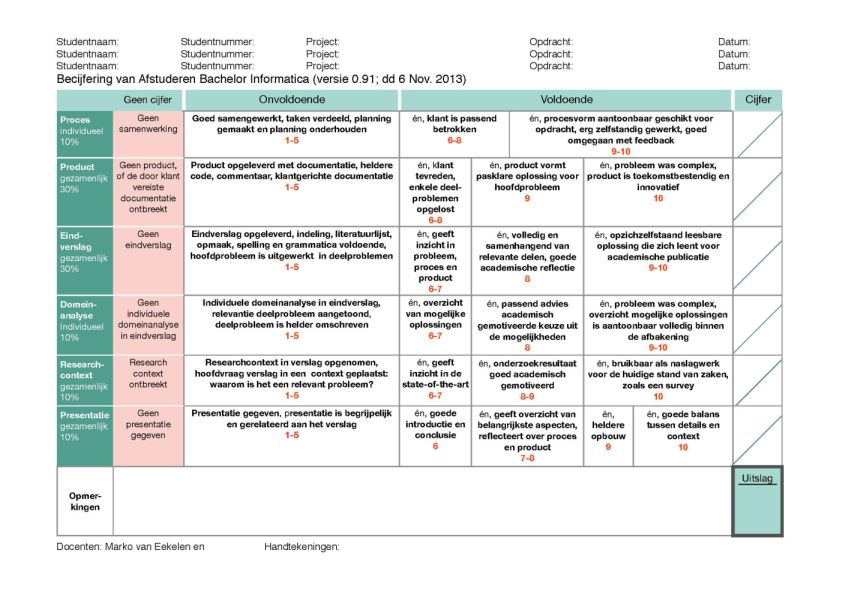
\includegraphics[width=.95\textwidth]{voorbeeld-ABI-cijfer.jpg}
	\captionof{figure}{Een voorbeeld voor bepaling van een ABI cijfer}
    \end{center}
\end{sidewaysfigure}

{\small\sf
\begin{center}
    \begin{tabular}{|p{7em}|p{23em}|}
	\hline
	{\bf eisen} & {\bf Criteria}\\\hline
	\multicolumn{2}{|c|}{\emph{Presenteren}}\\\hline
	Opbouw & De opbouw van de presentatie wordt duidelijk vermeld.
		Er wordt aangegeven welk teamlid welke rol in het project heeft vervuld en wie
		welk onderdeel van de presentatie zal verzorgen.
		Tijdens de presentatie is steeds duidelijk welke plaats het onderdeel in het
		geheel heeft.
	\\\hline
	Vormgeving & De bij de presentatie gebruikte hulpmiddelen (bv. Powerpoint) hebben een
		adequate vormgeving (kleurgebruik, hoeveelheid tekst per sheet, animaties, etc.)
	\\hline
	Communicatie & Er is duidelijkheid over de mogelijkheid tot het stellen van
		vragen, tijdens of na afloop van de presentatie. De vragen worden begrijpelijk beantwoord.
		De presentator(en) hebben de regie in handen.
	\\\hline
	Doelgroep & De presentatie is bedoeld voor de opdrachtgever, en moet dus aansluiten bij de
		achtergrondkennis van de opdrachtgever.
		De presentatie moet voor de opdrachtgever de relevante zaken over het  project
		duidelijk maken: wat is opgeleverd, hoe werkt het, welke onvolkomenheden bevat
		het systeem nog.
		De presentatie is ook goed te volgen voor stafleden van Informatica en
		gevorderde bachelor studenten.
	\\\hline
	\multicolumn{2}{|c|}{\emph{Klantgerichtheid}}\\\hline
	Rol van de opdrachtgever & De contacten met de opdrachtgever over de presentatie verlopen qua inhoud en
		planning zodanig dat deze weet wat er van de presentatie verwacht mag worden.
	\\\hline
	Overdracht & De overdracht van het resultaat van het project aan de klant gebeurt op zo’n
		manier dat de klant de resultaten daadwerkelijk kan gaan gebruiken.
	\\\hline
	\multicolumn{2}{|c|}{\emph{Schrijven scriptie}}\\\hline
	Taal & Het eindverslag is grammaticaal correct.
	\\\hline
	Precisie & De vereiste onderdelen komen voor in het verslag.
	\\\hline
	Structuur & De indeling van het verslag is helder.
		Er is samenhang tussen de tekstdelen.
	\\\hline
	Uitwerking probleemstelling & De probleemstelling is inhoudelijk
		verankerd in het onderzoek.
	\\\hline
	Presentatie vakinhoud & Het verslag maakt duidelijk hoe de opgeleverde producten van het project in
		relatie staan met de doelstelling van het project en de context van het onderzoek.
	\\\hline
    \end{tabular}
    \captionof{table}{Fase 4 Beoordelingscriteria eindpresentatie}
\end{center}
}% small sf


\end{document}
